\documentclass[hyperref={pdfpagelayout=SinglePage}]{beamer}

%Template
\usetheme{Warsaw}
\usecolortheme{default}
\usefonttheme[onlymath]{serif}

%Packages
\usepackage[utf8]{inputenc}
\usepackage[spanish,activeacute]{babel}
\usepackage{lipsum}
\usepackage{graphicx}
\usepackage{fancyhdr}
\usepackage{float}
\usepackage{adjustbox}
\usepackage{subfigure}
\usepackage{amsmath}
\usepackage{ragged2e}
\usepackage{color}
\usepackage{listings}
\usepackage{animate}
\usepackage{hyperref}

%Code
\lstset{ %
basicstyle=\small,       % the size of the fonts that are used for the code
numbers=none,                   % where to put the line-numbers
numberstyle=\footnotesize,      % the size of the fonts that are used for the line-numbers
stepnumber=1,                   % the step between two line-numbers. If it is 1 each line will be numbered
numbersep=5pt,                  % how far the line-numbers are from the code
backgroundcolor=\color{white},  % choose the background color. You must add \usepackage{color}
showspaces=false,               % show spaces adding particular underscores
showstringspaces=false,         % underline spaces within strings
showtabs=false,                 % show tabs within strings adding particular underscores
frame=single,           % adds a frame around the code
tabsize=4,          % sets default tabsize to N spaces
captionpos=b,           % sets the caption-position to bottom
breaklines=true,        % sets automatic line breaking
breakatwhitespace=false,    % sets if automatic breaks should only happen at whitespace
escapeinside={\%*}{*)}          % if you want to add a comment within your code
}

%Captions
\renewcommand{\lstlistingname}{Código}
\renewcommand\spanishtablename{Tabla}
\renewcommand{\figurename}{Gráfico}

%More
\makeatletter
\@addtoreset{subfigure}{framenumber}
\makeatother

\expandafter\def\expandafter\insertshorttitle\expandafter{%
  \insertshorttitle\hfill%
  \insertframenumber\,/\,\inserttotalframenumber}

\newcommand\Wider[2][5em]{%
\makebox[\linewidth][c]{%
  \begin{minipage}{\dimexpr\textwidth+#1\relax}
  \raggedright#2
  \end{minipage}%
  }%
}

%List of parts
\makeatletter
\AtBeginPart{%
    \addtocontents{parttoc}{\protect\beamer@partintoc{\the\c@part}{\beamer@partnameshort}{\the\c@page}}%
    \frame{\partpage}%
}
\newcommand{\parttableofcontents}{\@starttoc{parttoc}}
\newcommand{\beamer@partintoc}[3]{#2\par}
\makeatother

%Document Data
\title{Bosque de Obstáculos}
\subtitle{Trabajo Práctico Final}
\author{Badi Leonel, Buchhalter Nicolás Demián y Meola Franco Román}
\subject{Simulación de Sistemas}
\date{\today}

\begin{document}

\begin{frame}[plain]
    \frametitle{} 
    \titlepage
    \centering
	Grupo 3
\end{frame}

%Part List
%\begin{frame}
%\frametitle{Que vamos a ver}
%\parttableofcontents
%\end{frame}

%First Part
%\part{Egreso de una habitación}

\section{Fundamentos}

\subsection{Introducción}

\begin{frame}
\frametitle{Introducción}
\begin{itemize}
	\item Vamos a simular peatones que viajarán desde un punto inicial a un punto final.
	\item Estos están equipados con un mecanismo de navegación necesario para evitar colisiones con obstáculos fijos.
	\item Utilizaremos el \textit{Contractile Particle Model}.
	\item Implementación propia (No se utilizaron plataformas de simulación peatonal).
\end{itemize}
\end{frame}

\subsection{Objetivos}

\begin{frame}
\frametitle{Objetivos}
\begin{block}{Definición de una heurística}
Crear una heurística que permita ajustar \textbf{dinámicamente} el ángulo del versor de la velocidad deseada en función de las posiciones de los ángulos.
\end{block}
\begin{exampleblock}{Para los obstáculos fijos (los árboles)}
Se pueden \textbf{precalcular} de antemano los mejores caminos para todos los agentes.
\end{exampleblock}
\begin{alertblock}{Para los obstáculos móviles (los otros agentes)}
Se deberá agregar un nuevo componente al modelo para anticipar la colisión entre agentes.
\end{alertblock}
\end{frame}

\subsection{Estado del Arte}

\begin{frame}
\frametitle{Estado del Arte}
\begin{itemize}
	\item Lorem.
	\item Lorem.
	\item Lorem.
\end{itemize}
\end{frame}

\section{Implementación}

\subsection{Sistema}

\begin{frame}
\frametitle{Sistema}
\framesubtitle{Agentes}
\begin{itemize}
	\item $N = 300$
	\item $r_{min} = 0.15m$
	\item $r_{max} = 0.32m$
	\item $v_{d}^{max} = 1.55 \frac{m}{s}$
\end{itemize}
\end{frame}

\begin{frame}
\frametitle{Sistema}
\framesubtitle{Escena}
\begin{itemize}
	\item $A$ obstáculos fijos (árboles) distribuidos aleatoriamente.
	\item Lorem.
	\item Lorem.
	\item \textbf{Dimensiones:}
	\begin{itemize}
		\item Habitación rectangular de $Xm$ x $Xm$.
		\item Puerta central de $Xm$ de apertura.
	\end{itemize}
\end{itemize}
\end{frame}

\begin{frame}
\frametitle{Sistema}
\framesubtitle{Escena}
\begin{figure}[H]
	\centering
    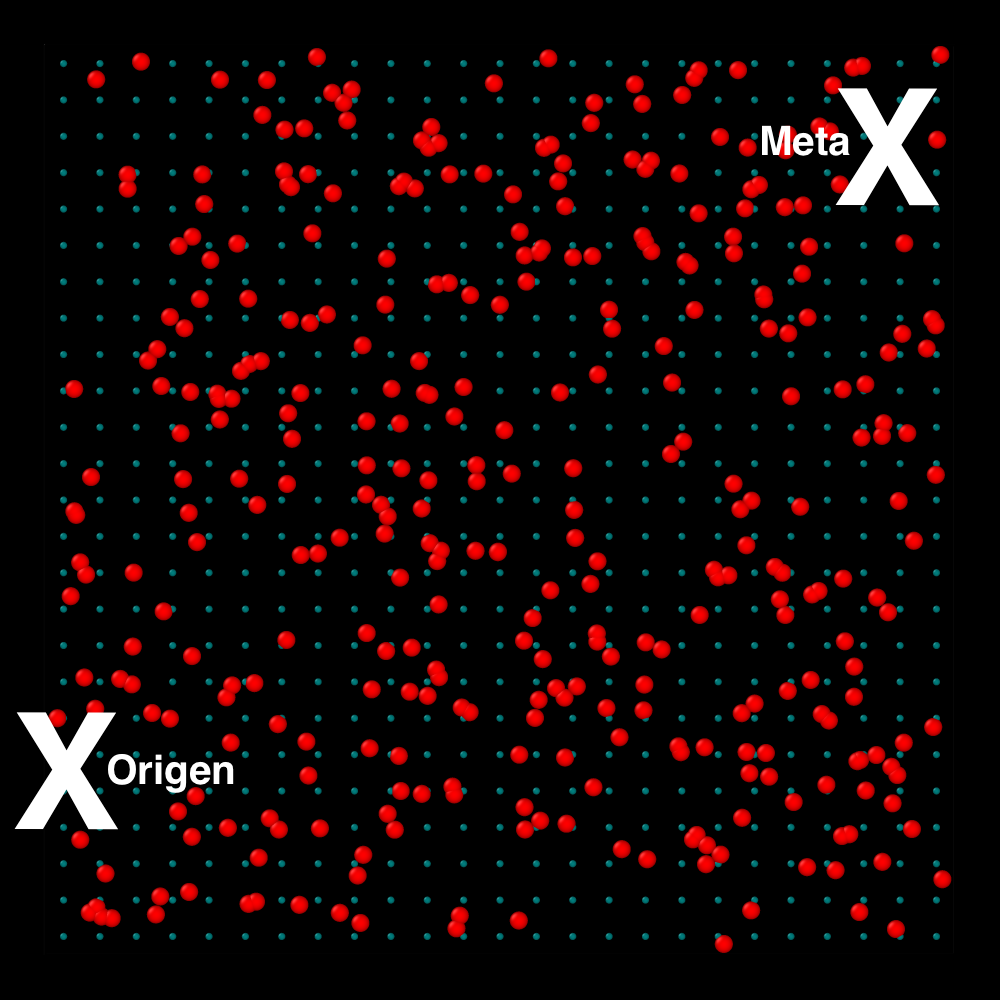
\includegraphics[width=0.75\textwidth]{images/scene.png}
    \caption{Esquema del sistema de obstáculos fijos con posiciones inicial y final de un peatón simulado.}
\end{figure}
\end{frame}

\begin{frame}
\frametitle{Sistema}
\framesubtitle{Modelo}
\begin{itemize}
	\item \textbf{Parámetros del \textit{Contractile Particle Model}:}
	\begin{itemize}
		\item $\tau = 0.5s$
		\item $\beta = 0.9$
	\end{itemize}
\end{itemize}
\end{frame}

\subsection{Heurística}

\begin{frame}
\frametitle{Heurística}
\framesubtitle{Subtítulo 1}
\begin{itemize}
	\item Lorem
	\item Lorem
	\item Lorem
\end{itemize}
\end{frame}

\begin{frame}
\frametitle{Heurística}
\framesubtitle{Subtítulo 2}
\begin{itemize}
	\item Lorem
	\item Lorem
	\item Lorem
\end{itemize}
\end{frame}

\subsection{Simulación}

\begin{frame}
\frametitle{Simulación}
\framesubtitle{Variables relevantes de la simulación}
\begin{itemize}
	\item $t$ $[s]$: Tiempo (en segundos) a visualizar.
	\item $dt$ $[s]$: Tiempo (en segundos) del paso de la simulación.
	\item $k$: Relación entre cantidad de pasos simulados y escritos para visualización.
\end{itemize}
\end{frame}

\begin{frame}[fragile]
\frametitle{Simulación}
\framesubtitle{Algoritmo de simulación}
\begin{lstlisting}[language=Java, caption = Algoritmo de simulación]
public void simulate(double t, double dt, int k){
	writeFrame(0);
	int framesWrited = 1;
	double totalTimeSimulated = 0;
	moveSystem(dt);
	totalTimeSimulated += dt;
	while(totalTimeSimulated < t){
		for(int i = 0; i < k; i++){
			moveSystem(dt);
			totalTimeSimulated += dt;
		}
		writeFrame(framesWrited++);
	}
}
\end{lstlisting}
\end{frame}

\begin{frame}
\frametitle{Simulación}
\framesubtitle{Variables relevantes de la simulación}
\begin{itemize}
	\item \textbf{Parámetros de la simulación:}
	\begin{itemize}
		\item $k = 5$
		\item $dt = 0.05s$
	\end{itemize}
\end{itemize}
\end{frame}

\begin{frame}
\frametitle{Simulación}
\framesubtitle{Detalles de implementación}
\begin{itemize}
	\item Se implementó un modelo que contempla una lista de \textit{targets} para cada una de las partículas.
	\item Lorem.
	\item Lorem \textit{Cell Index Method} Lorem.
\end{itemize}
\end{frame}

\begin{frame}
\frametitle{Simulación}
\framesubtitle{Visualización}
\begin{itemize}
	\item La simulación y la visualización son independientes
	\item El algoritmo de simulación escribe un archivo \texttt{.tsv} con los siguientes datos:
	\begin{itemize}
		\item $(x,y)$
		\item $r$
		\item Color RGB para indicar las velocidades, donde R es la componente en el eje Y y G es la componente en eje X
	\end{itemize}
	\item Por último, se carga en \texttt{Ovito} el archivo de salida\texttt{.tsv} para realizar la visualización
\end{itemize}
\end{frame}

\section{Resultados}

\subsection{Gráficos y Tablas}

\begin{frame}
\Wider{
\frametitle{Gráfico de ?}
\framesubtitle{Para $? = ?$}
\begin{figure}[H]
	\centering
    \includegraphics[width=\textwidth]{example-image}
\end{figure}
}
\end{frame}

\begin{frame}
\frametitle{Tabla de ?}
\framesubtitle{Para distintos valores de ?}
\begin{center}
\begin{table}[h]
\centering
\adjustbox{max height=\dimexpr\textheight-3.0cm\relax,
           max width=\textwidth}{
\begin{tabular}{cc}
\hline
\textbf{?} & \textbf{?}\\ \hline
?&?\\ 
\end{tabular}
}
\caption{? para distintos valores de ?}
\end{table}
\end{center}
\end{frame}

\subsection{Animaciones}

\begin{frame}[plain]
\frametitle{Animación de la simulación}
\framesubtitle{Para $? = ?$}
\begin{figure}[H]
	\centering
%	\animategraphics[loop,controls,width=0.85\textwidth]{10}{animation/300n}{00001}{00242}
\end{figure}
\end{frame}

\subsection{Conclusiones}

\begin{frame}
\frametitle{Conclusiones}
\begin{itemize}
	\item Lorem
	\item Lorem
	\item Lorem
\end{itemize}	
\end{frame} 

\begin{frame}[plain]
    \centering
	\Huge Gracias
\end{frame}

\end{document}
